\documentclass[11pt]{article}

% Supplementary Material for
% "Equilibrium Bifurcations and Periodic Dynamics in a Planar Restricted
%  Five-Body Problem with Four Unequal Primaries"
% Tables/figures are AUTO-GENERATED from the verified result CSVs.

\usepackage[margin=1in]{geometry}
\usepackage{amsmath,amssymb}
\usepackage{graphicx}
\usepackage{booktabs}
\usepackage[hidelinks]{hyperref}

\graphicspath{{figures/}}

\newcommand{\Om}{\Omega}
\newcommand{\grad}{\nabla}
\newcommand{\CJ}{C_J}

\renewcommand{\thesection}{S\arabic{section}}
\renewcommand{\thetable}{S\arabic{table}}
\renewcommand{\thefigure}{S\arabic{figure}}

\title{Supplementary Material\\
\large Equilibrium Bifurcations and Periodic Dynamics in a Planar Restricted
Five-Body Problem with Four Unequal Primaries}
\author{Muhammad Shoaib \and A.~R.~Kashif}
\date{\today}

\begin{document}
\maketitle

This document collects material supporting the main text: the refinement
displacements and full recomputed equilibrium coordinates of the reference
cases, the Cartesian branch diagrams, the complete set of local fold panels, the
remaining periodic-orbit family figures and candidate ranking, the individual
centre frequencies, and a summary of numerical-robustness checks. All tables and
figures are generated from the same result files as the main text.

\section{Baseline configurations}
The four representative baseline configurations with their computed equilibria
(the counts $5,9,5,5$ are established in the main text).
\begin{figure}[htbp]\centering
  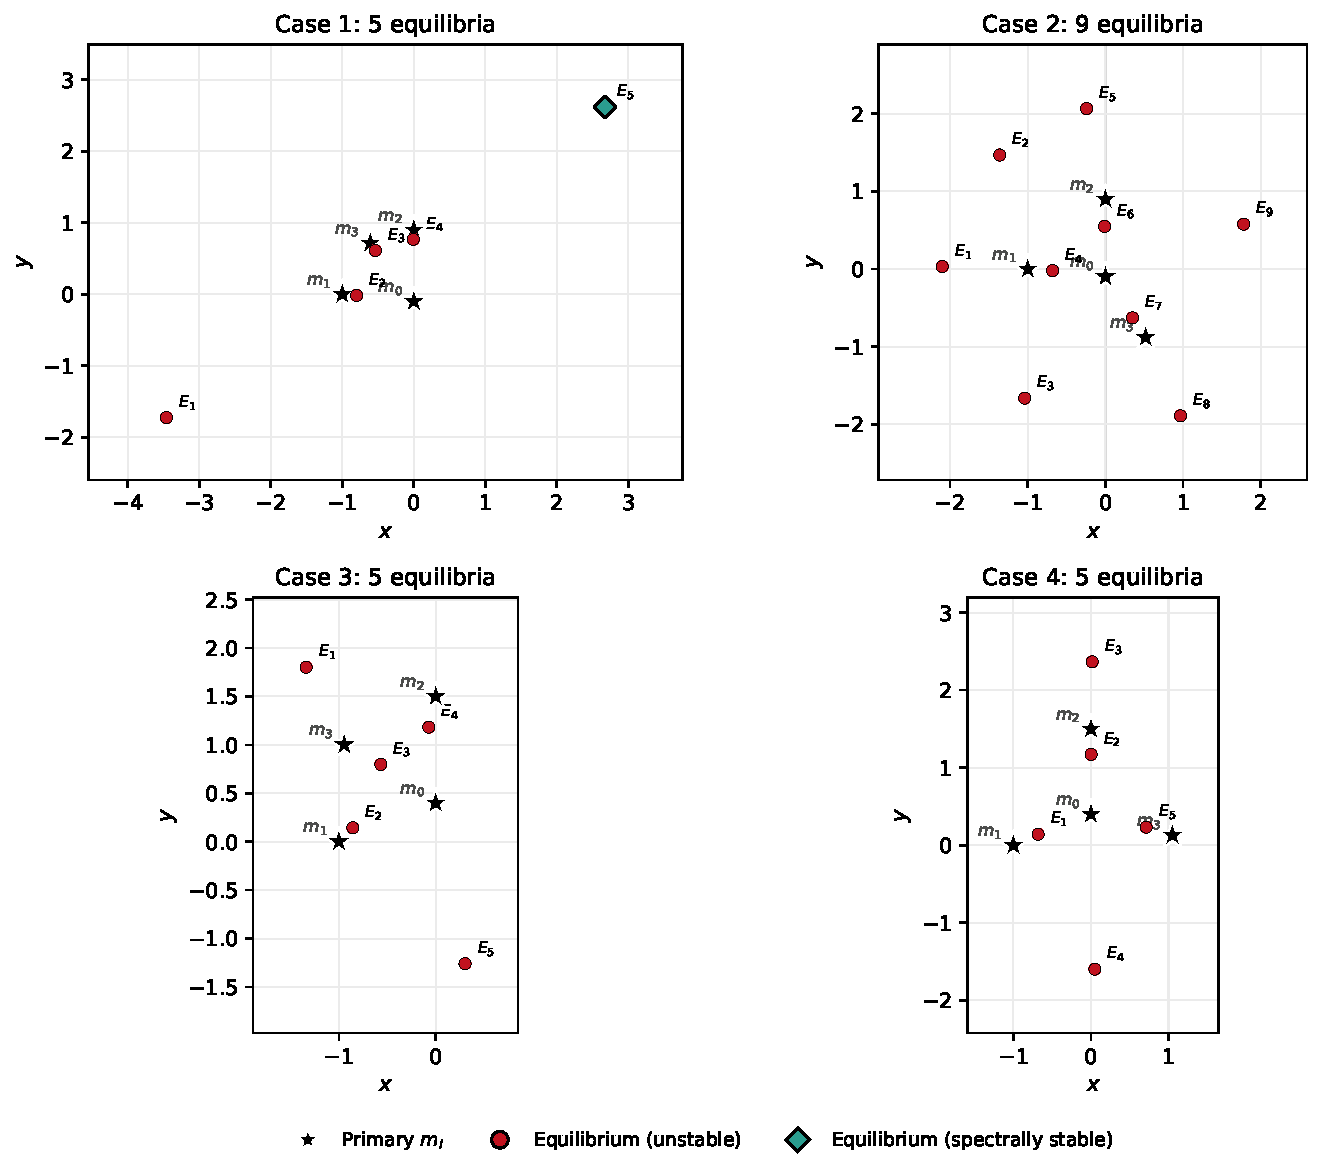
\includegraphics[width=\textwidth]{verified_cases_equilibria.pdf}
  \caption{The four baseline configurations. Black stars: primaries at their
  refined positions; filled circles: equilibria located independently
  ($\|\grad\Om\|<10^{-12}$); one Case-1 equilibrium near $(2.67,2.62)$ (green
  diamond) is spectrally stable.}
\end{figure}

\section{Refinement of the baseline configurations}
Displacements used to project each configuration onto $\psi=0$ (holding
$a,b$ fixed); the adopted single-coordinate move, the alternative
single-coordinate move, and the distance to the constrained nearest CC point
(both coordinates free).
% AUTO-GENERATED by paper/make_tables.py from results/*.csv. Do not edit by hand.
\begin{table}[t]
\centering
\caption{Refinement of each approximate configuration onto $\psi=0$. The single coordinate with the smaller displacement is adopted; the alternative single-coordinate displacements and the distance to the constrained nearest CC point (both coordinates free) are listed for transparency.}
\label{tab:refinement}
\small
\begin{tabular}{lccccccc}
\toprule
Case & var & $\Delta$ & $|\psi|_{\mathrm{before}}$ & $|\psi|_{\mathrm{after}}$ & $\Delta c_1^{\mathrm{opt}}$ & $\Delta c_2^{\mathrm{opt}}$ & min-norm \\
\midrule
Case 1 & $c2$ & $5.7\times10^{-3}$ & $6.0\times10^{-3}$ & $8.8\times10^{-17}$ & $-1.2\times10^{-2}$ & $5.7\times10^{-3}$ & $5.1\times10^{-3}$ \\
Case 2 & $c1$ & $-2.3\times10^{-3}$ & $9.2\times10^{-3}$ & $9.5\times10^{-15}$ & $-2.3\times10^{-3}$ & $4.0\times10^{-3}$ & $2.0\times10^{-3}$ \\
Case 3 & $c1$ & $1.5\times10^{-2}$ & $7.4\times10^{-2}$ & $3.6\times10^{-15}$ & $1.5\times10^{-2}$ & $2.8\times10^{-2}$ & $1.5\times10^{-2}$ \\
Case 4 & $c1$ & $5.8\times10^{-4}$ & $3.4\times10^{-2}$ & $3.6\times10^{-15}$ & $5.8\times10^{-4}$ & $-1.9\times10^{-3}$ & $5.6\times10^{-4}$ \\
\bottomrule
\end{tabular}
\end{table}


\section{Full equilibrium coordinates}
Every computed equilibrium of the four baseline configurations, with gradient
residual, Hessian determinant, adopted Jacobi value, and linear-stability
classification.
% AUTO-GENERATED by paper/make_tables.py from results/*.csv. Do not edit by hand.
\begin{table}[t]
\centering
\caption{Independently recomputed equilibria at the refined configurations. Each root satisfies $\|\nabla\Omega\|<10^{-12}$. $D=\det \mathrm{H}\Omega=\Omega_{xx}\Omega_{yy}-\Omega_{xy}^2$; $C_J=2\Omega$ is the adopted Jacobi value at the equilibrium; $\max\operatorname{Re}\lambda$ is taken over the four eigenvalues of the variational matrix. `Unstable' denotes $\max\operatorname{Re}\lambda>10^{-8}$; `spectrally stable' denotes a purely imaginary spectrum (linear statement only).}
\label{tab:equilibria}
\footnotesize
\setlength{\tabcolsep}{4pt}
\begin{tabular}{llrrccrl}
\toprule
Case & $i$ & $x$ & $y$ & $\|\nabla\Omega\|$ & $D$ & $\max\operatorname{Re}\lambda$ & class \\
\midrule
Case 1 & 1 & $-3.46033$ & $-1.72387$ & $<\!10^{-16}$ & $-0.069$ & $0.2587$ & unstable \\
Case 1 & 2 & $-0.79965$ & $-0.01525$ & $1.3\times10^{-14}$ & $-4.5\times10^{5}$ & $30.84$ & unstable \\
Case 1 & 3 & $-0.53766$ & $0.61300$ & $3.5\times10^{-14}$ & $-6.3\times10^{5}$ & $33.73$ & unstable \\
Case 1 & 4 & $-0.00736$ & $0.76860$ & $4.3\times10^{-14}$ & $-6.6\times10^{5}$ & $34.02$ & unstable \\
Case 1 & 5 & $2.67101$ & $2.62208$ & $<\!10^{-16}$ & $0.0826$ & $2.0\times10^{-15}$ & spectrally stable \\
\midrule
Case 2 & 1 & $-2.10151$ & $0.03278$ & $9.5\times10^{-16}$ & $-0.934$ & $0.8291$ & unstable \\
Case 2 & 2 & $-1.36116$ & $1.46813$ & $2.2\times10^{-16}$ & $0.6338$ & $0.442$ & unstable \\
Case 2 & 3 & $-1.03954$ & $-1.66117$ & $2.2\times10^{-16}$ & $0.6261$ & $0.415$ & unstable \\
Case 2 & 4 & $-0.68050$ & $-0.01961$ & $6.3\times10^{-15}$ & $-3483$ & $9.132$ & unstable \\
Case 2 & 5 & $-0.24287$ & $2.06612$ & $2.8\times10^{-17}$ & $-0.7812$ & $0.7738$ & unstable \\
Case 2 & 6 & $-0.01142$ & $0.54921$ & $1.1\times10^{-15}$ & $-3976$ & $9.426$ & unstable \\
Case 2 & 7 & $0.34816$ & $-0.62794$ & $1.2\times10^{-15}$ & $-5549$ & $10.22$ & unstable \\
Case 2 & 8 & $0.96571$ & $-1.88879$ & $4.6\times10^{-16}$ & $-1.196$ & $0.9031$ & unstable \\
Case 2 & 9 & $1.77904$ & $0.57872$ & $2.2\times10^{-16}$ & $0.6822$ & $0.409$ & unstable \\
\midrule
Case 3 & 1 & $-1.33841$ & $1.80166$ & $<\!10^{-16}$ & $-3.041$ & $1.323$ & unstable \\
Case 3 & 2 & $-0.85640$ & $0.14392$ & $2.0\times10^{-15}$ & $-812.6$ & $6.483$ & unstable \\
Case 3 & 3 & $-0.56675$ & $0.79837$ & $1.2\times10^{-15}$ & $-824.2$ & $6.385$ & unstable \\
Case 3 & 4 & $-0.07178$ & $1.18250$ & $2.2\times10^{-15}$ & $-516.2$ & $5.794$ & unstable \\
Case 3 & 5 & $0.30292$ & $-1.25995$ & $2.3\times10^{-16}$ & $0.7515$ & $0.3409$ & unstable \\
\midrule
Case 4 & 1 & $-0.68158$ & $0.14200$ & $2.3\times10^{-15}$ & $-2333$ & $8.207$ & unstable \\
Case 4 & 2 & $0.00194$ & $1.17180$ & $1.1\times10^{-15}$ & $-1742$ & $7.634$ & unstable \\
Case 4 & 3 & $0.01572$ & $2.36548$ & $<\!10^{-16}$ & $-3.379$ & $1.32$ & unstable \\
Case 4 & 4 & $0.05059$ & $-1.59719$ & $2.5\times10^{-16}$ & $0.9505$ & $0.442$ & unstable \\
Case 4 & 5 & $0.71196$ & $0.23320$ & $3.8\times10^{-15}$ & $-2222$ & $8.11$ & unstable \\
\bottomrule
\end{tabular}
\end{table}


\section{Cartesian branch diagrams}
The Cartesian branch coordinates $x_i(s)$ and $y_i(s)$ along the two admissible
arcs (the radial coordinate $r_i(s)$ is in the main text). They show the same
fold and mass-vanishing events.
\begin{figure}[htbp]\centering
  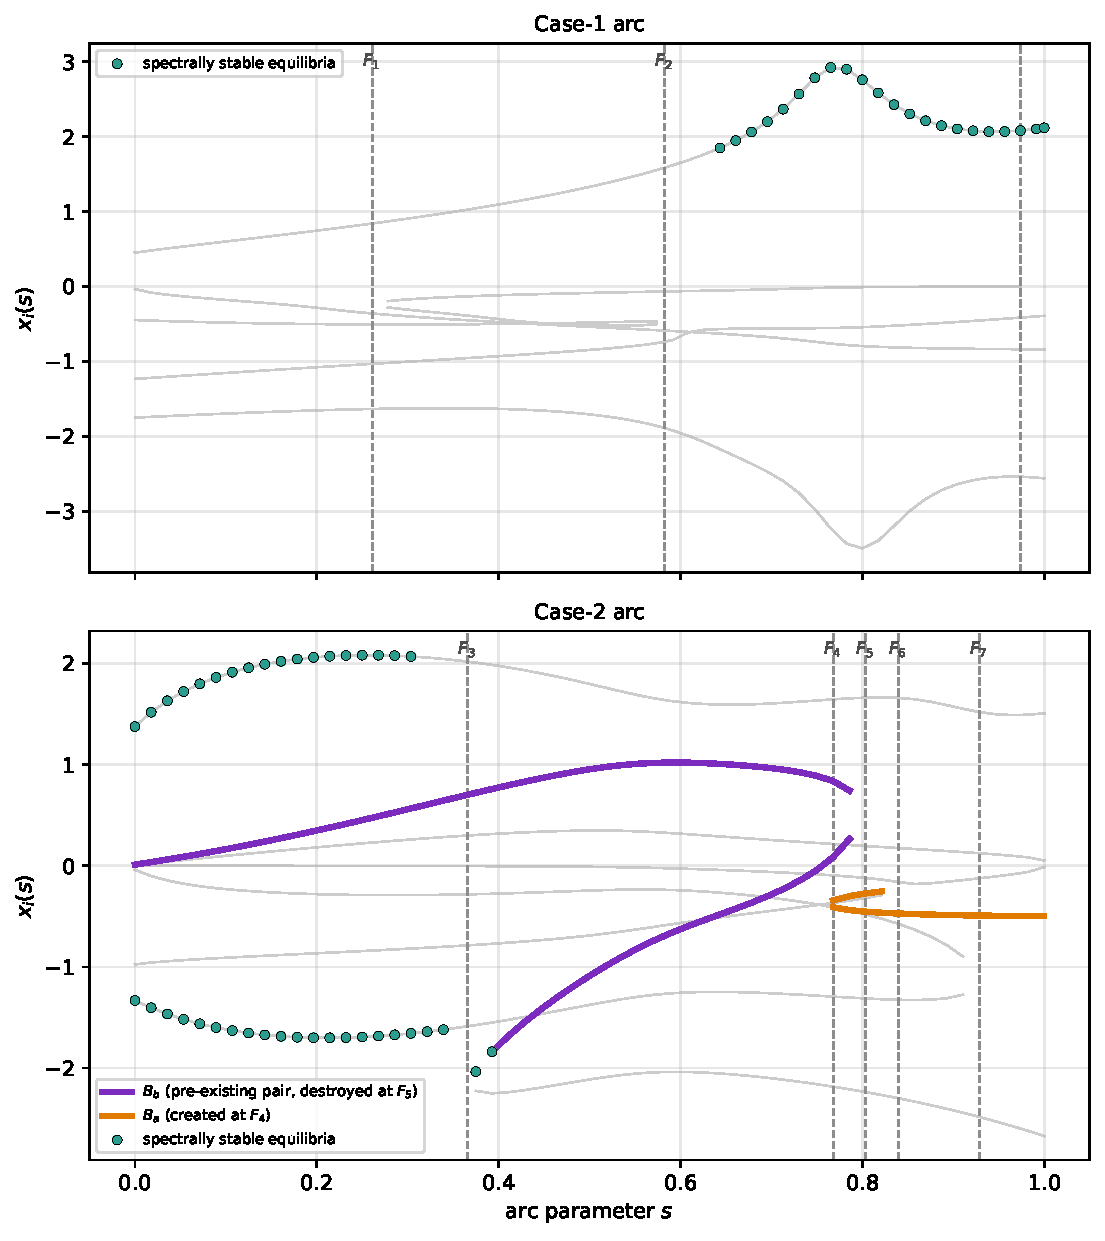
\includegraphics[width=\textwidth]{equilibrium_branches_x_vs_s.pdf}
  \caption{Branch coordinate $x_i(s)$; dashed verticals mark the folds.}
\end{figure}
\begin{figure}[htbp]\centering
  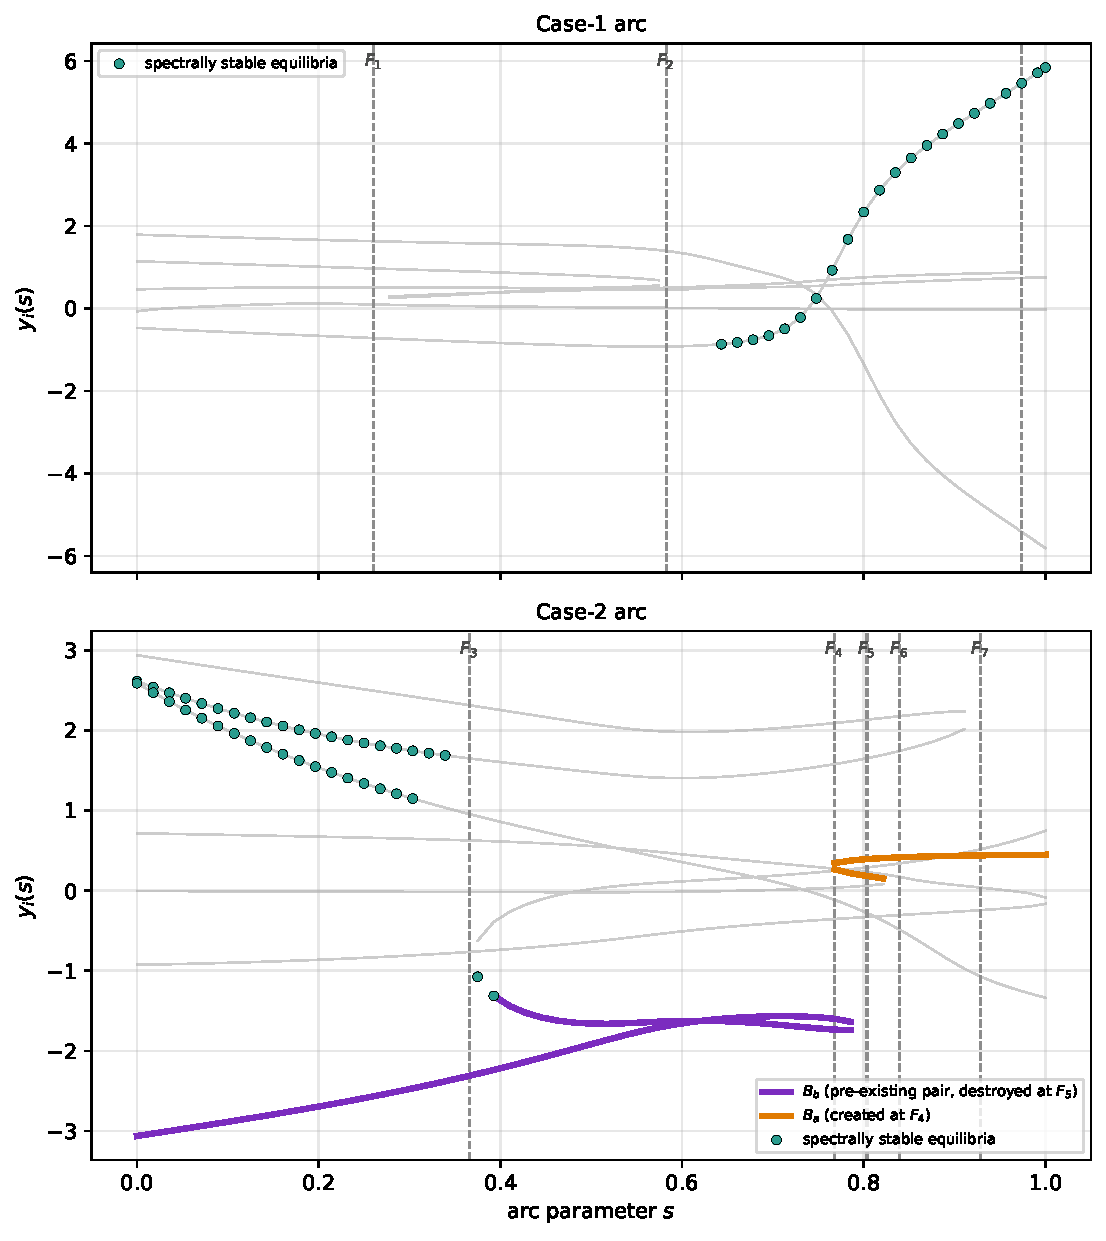
\includegraphics[width=\textwidth]{equilibrium_branches_y_vs_s.pdf}
  \caption{Branch coordinate $y_i(s)$; dashed verticals mark the folds.}
\end{figure}

\section{Local panels for all seven folds}
Local structure of every interior saddle-node: the $x$-coordinates of the
merging pair against arclength $\ell-\ell_c$ (three representatives appear in
the main text).
\begin{figure}[htbp]\centering
  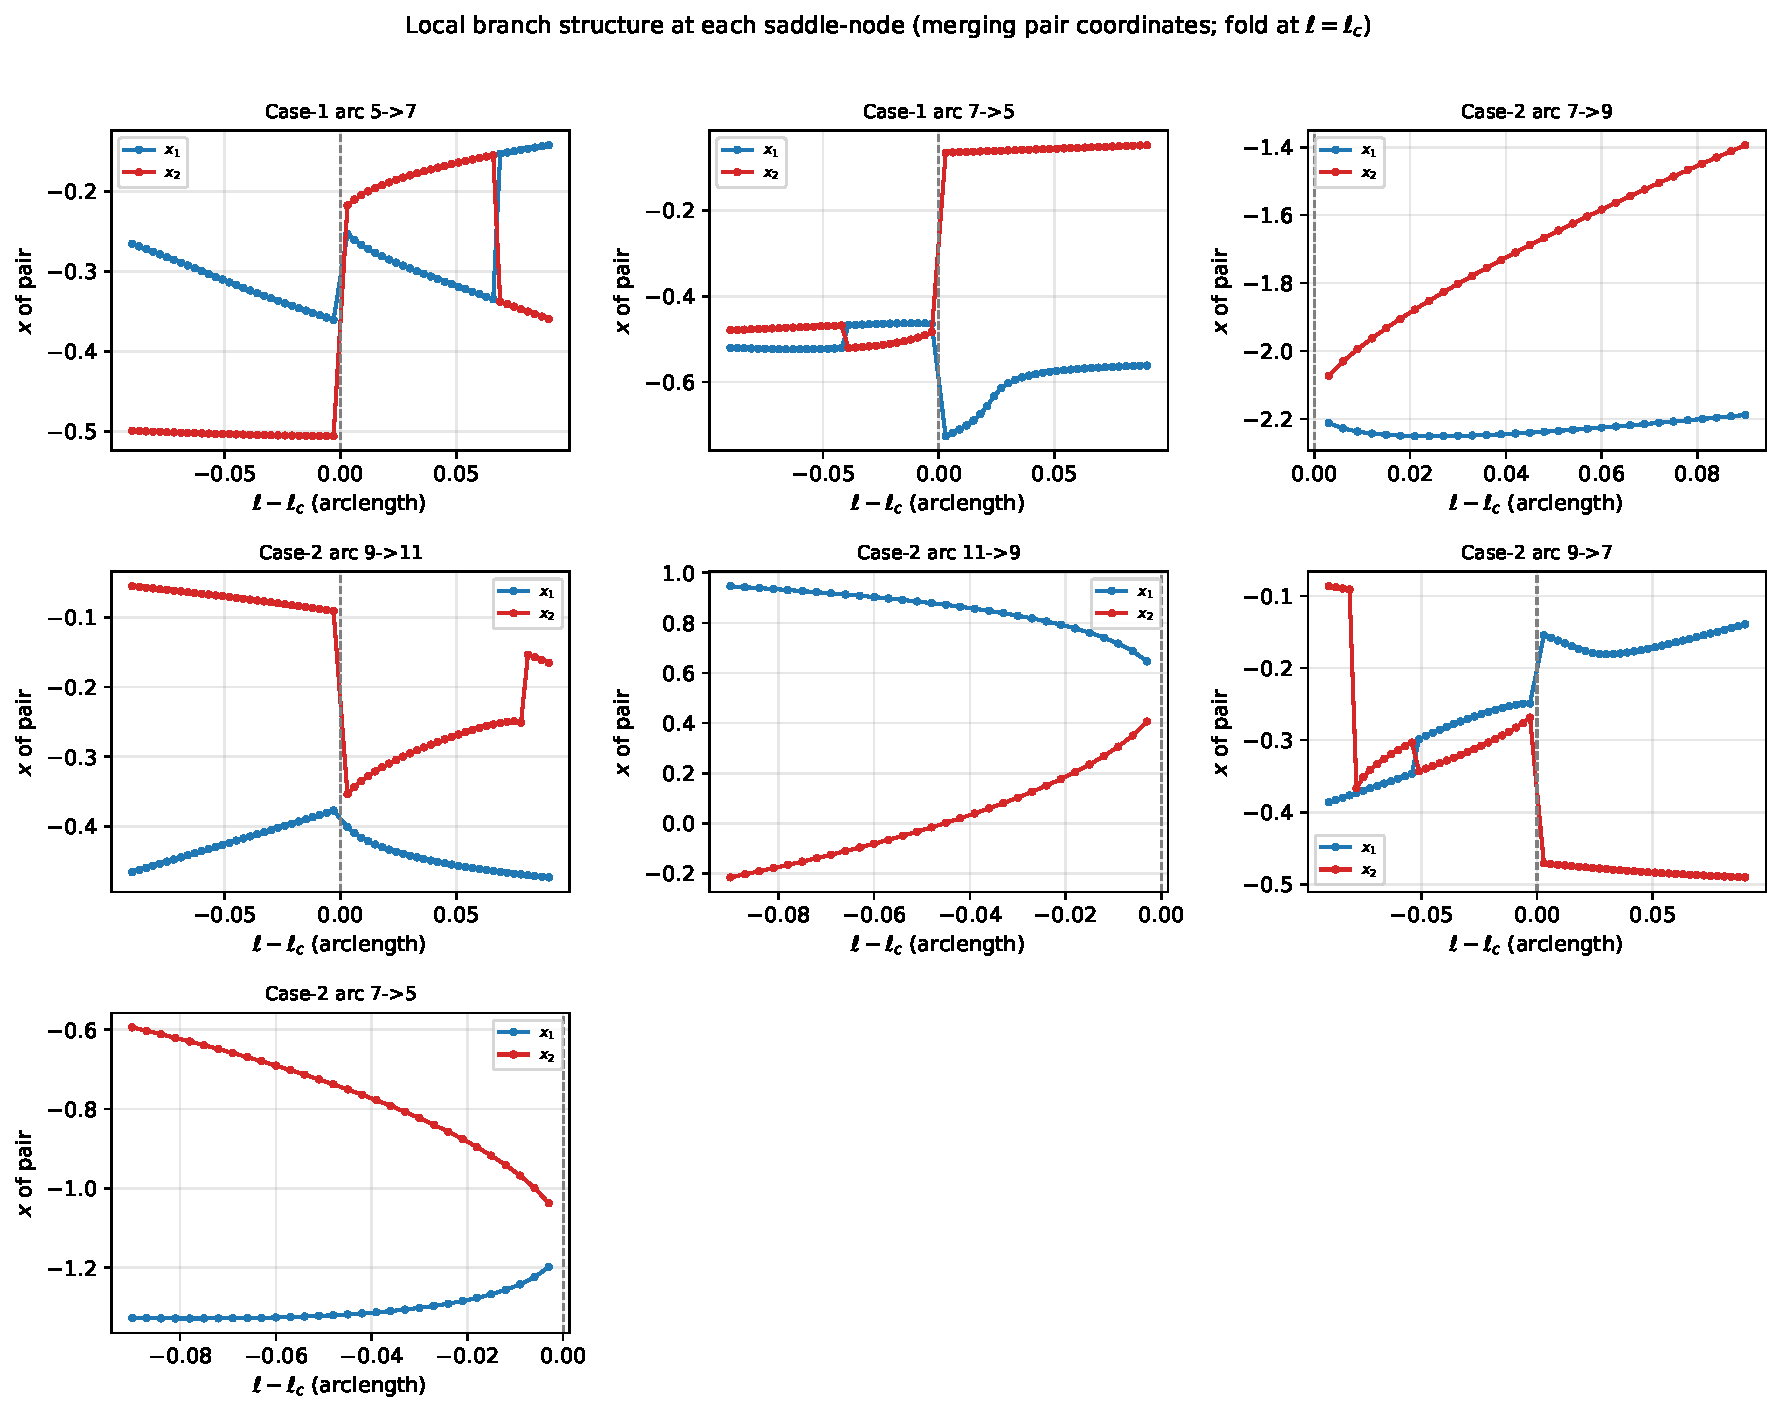
\includegraphics[width=\textwidth]{fold_zoom_branches.pdf}
  \caption{Merging-pair coordinates at all seven folds; the pair annihilates at
  $\ell=\ell_c$ (dashed).}
\end{figure}

\section{Additional periodic-orbit families}
The two stable Lyapunov families not shown in the main text.
\begin{figure}[htbp]\centering
  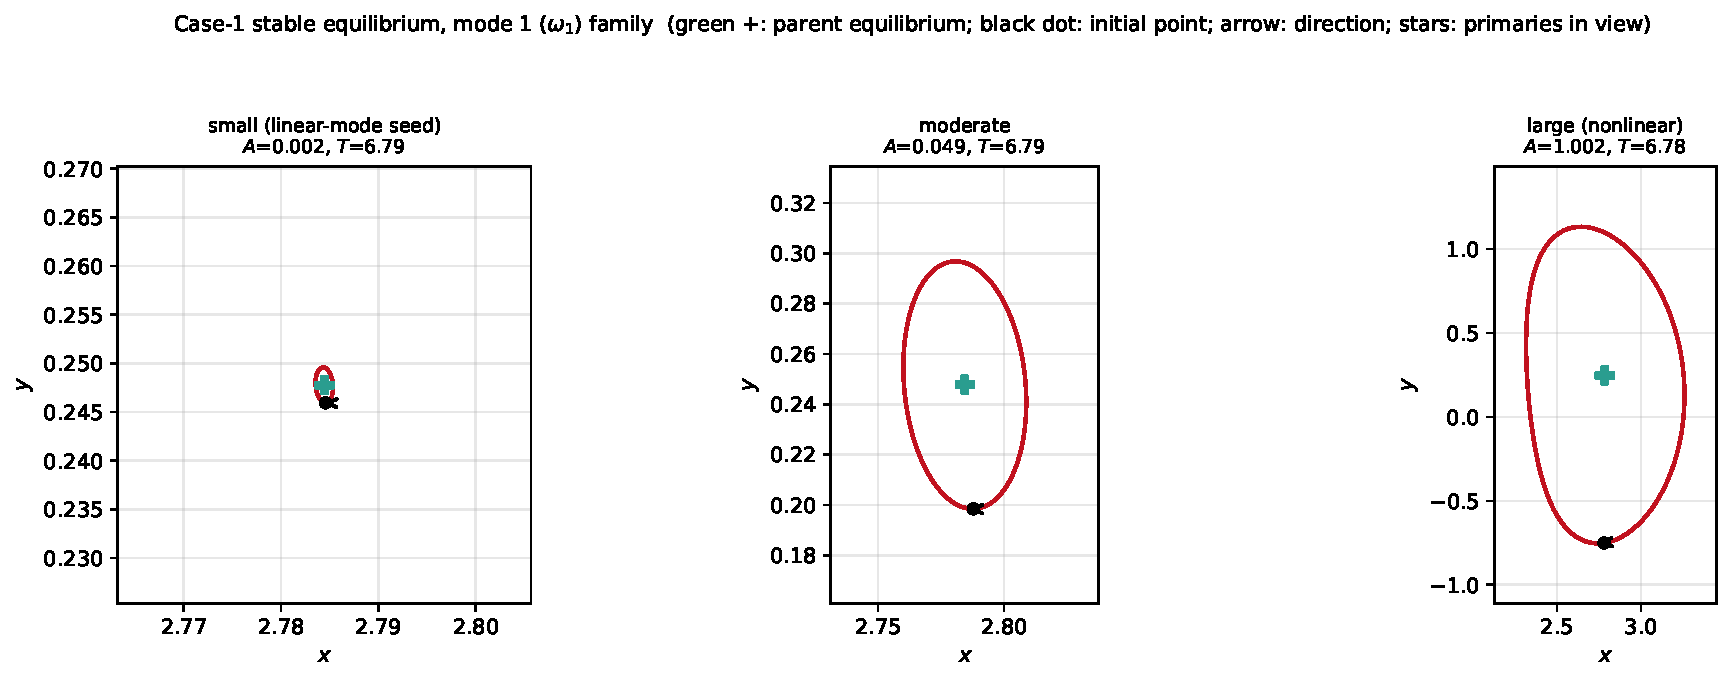
\includegraphics[width=\textwidth]{periodic_family_case1_mode1.pdf}
  \caption{Case-1 arc stable equilibrium, mode-1 ($\omega_1$) family.}
\end{figure}
\begin{figure}[htbp]\centering
  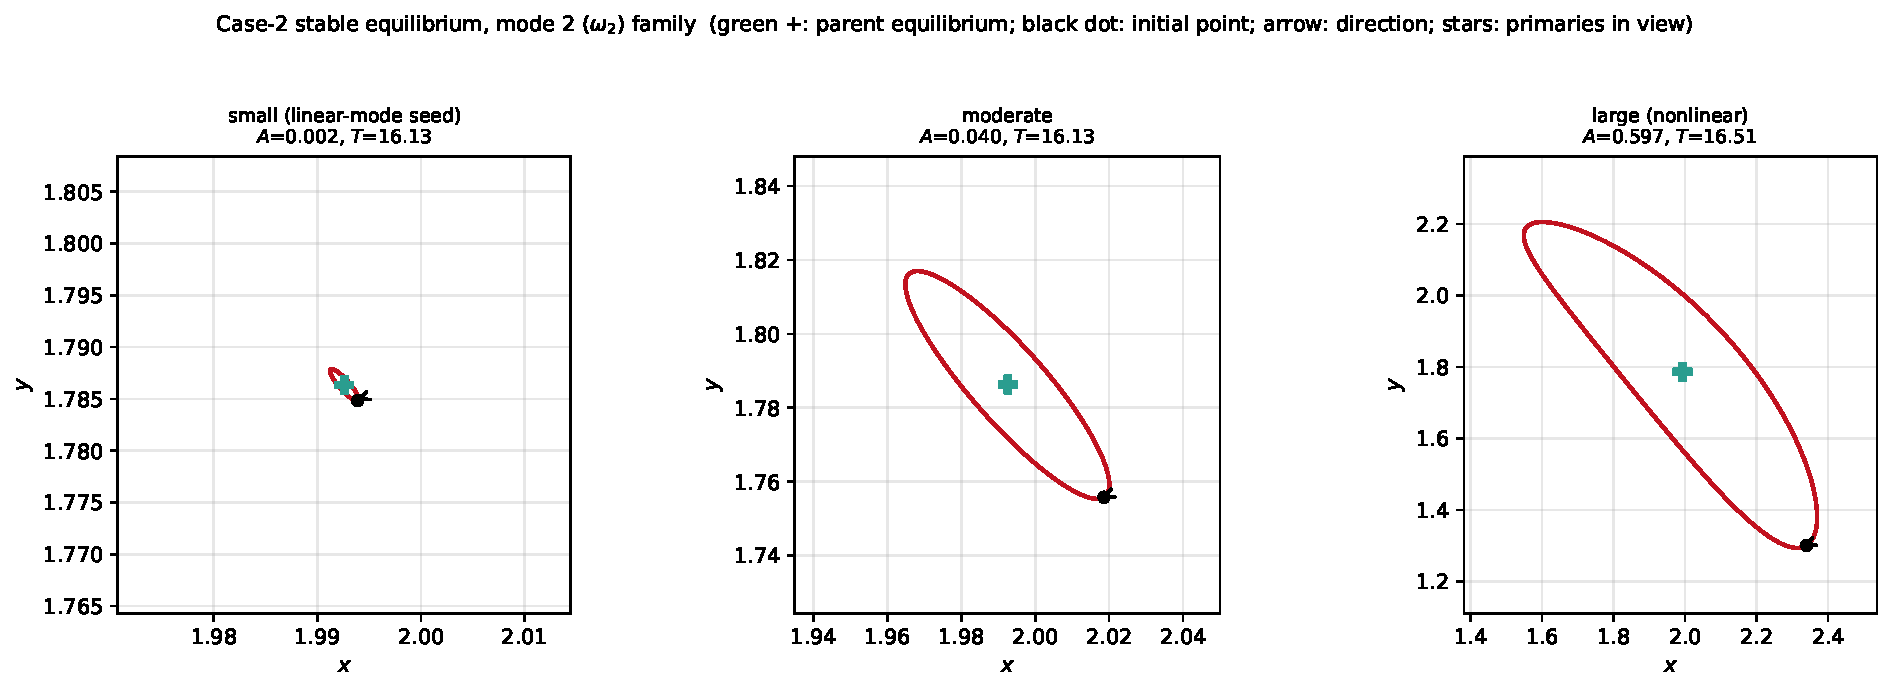
\includegraphics[width=\textwidth]{periodic_family_case2_mode2.pdf}
  \caption{Case-2 arc stable equilibrium, mode-2 ($\omega_2$) family.}
\end{figure}

\section{Individual centre frequencies}
\begin{figure}[htbp]\centering
  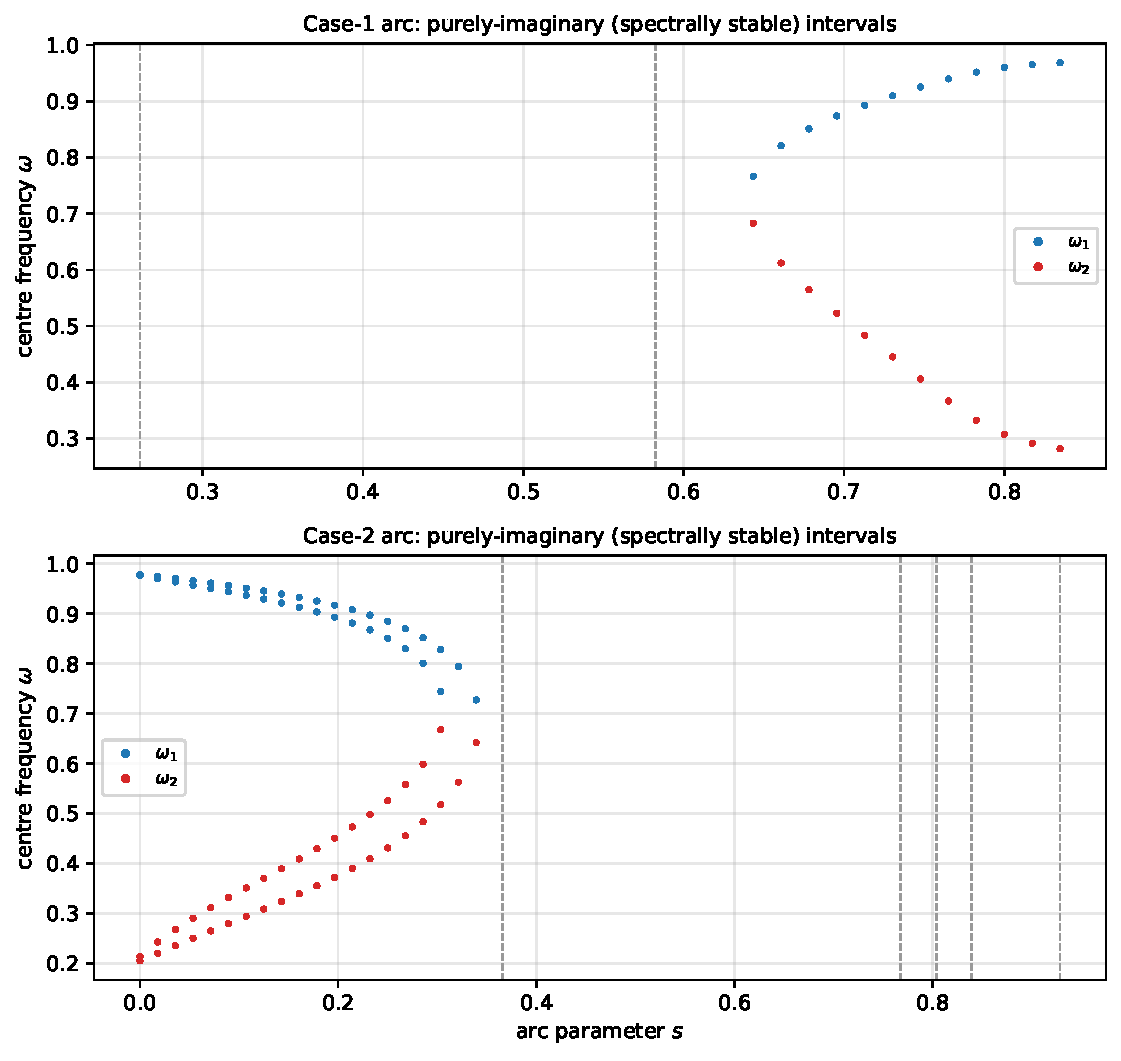
\includegraphics[width=\textwidth]{centre_frequencies_vs_s.pdf}
  \caption{Centre frequencies $\omega_1\ge\omega_2$ on the spectrally stable
  intervals of each arc; dashed verticals mark folds.}
\end{figure}

\section{Stable versus unstable orbit on the Hill geometry}
\begin{figure}[htbp]\centering
  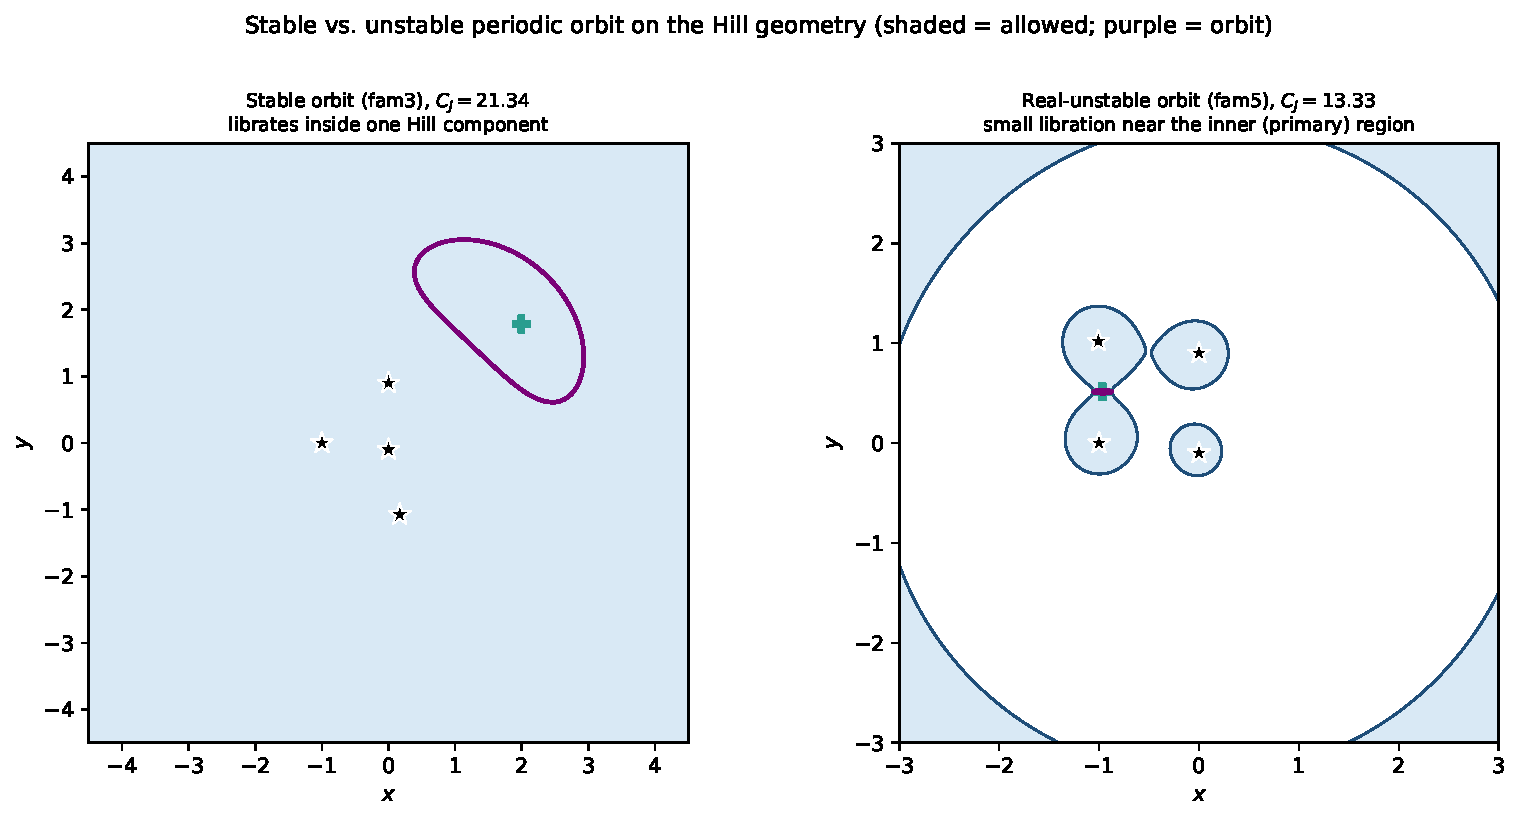
\includegraphics[width=0.95\textwidth]{hill_stable_vs_unstable.pdf}
  \caption{A Floquet-stable orbit (left, fam~3) and a real-unstable orbit
  (right, fam~5) on their respective Hill geometries at their own $\CJ$ (shaded:
  allowed; blue: zero-velocity curve; purple: orbit; stars: primaries; green
  $+$: parent equilibrium).}
\end{figure}

\section{Ranked centre-mode candidates}
The centre-mode intervals ranked as periodic-orbit continuation candidates
(the computed families are summarized in the main text).
% AUTO-GENERATED by paper/make_tables.py from results/*.csv. Do not edit by hand.
\begin{table}[t]
\centering
\caption{Top-ranked centre-mode equilibria for future periodic-orbit continuation (ranked by centre-mode interval width, favouring purely-imaginary spectra). `centre2' denotes a spectrally stable (two-centre) interval; `saddle$\times$centre' a single centre pair. $\omega_1,\omega_2$ are centre frequencies at the representative point; $C_J=2\Om$. Eigenvectors and continuation parameters $(c_1,c_2,s)$ for each are stored in \texttt{results/periodic\_orbit\_candidates.csv}.}
\label{tab:pocands}
\footnotesize
\setlength{\tabcolsep}{4pt}
\begin{tabular}{clccccc}
\toprule
rank & arc / type & $s$-interval & $(c_1,c_2)_{\mathrm{rep}}$ & $\omega_1$ & $\omega_2$ & $C_J$ \\
\midrule
1 & Case-1 arc (s$\times$c) & $[0.000,1.000]$ & $(-0.884,0.886)$ & $4.284$ & -- & $19.855$ \\
2 & Case-2 arc (s$\times$c) & $[0.000,1.000]$ & $(0.512,-0.888)$ & $7.435$ & -- & $24.294$ \\
3 & Case-1 arc (s$\times$c) & $[0.000,1.000]$ & $(-0.884,0.886)$ & $4.939$ & -- & $20.768$ \\
4 & Case-2 arc (s$\times$c) & $[0.000,1.000]$ & $(0.512,-0.888)$ & $6.861$ & -- & $24.544$ \\
5 & Case-2 arc (s$\times$c) & $[0.000,0.911]$ & $(0.487,-0.919)$ & $1.113$ & -- & $13.095$ \\
6 & Case-1 arc (s$\times$c) & $[0.000,0.835]$ & $(-0.953,0.960)$ & $1.351$ & -- & $11.550$ \\
7 & Case-2 arc (s$\times$c) & $[0.000,0.821]$ & $(0.442,-0.959)$ & $8.375$ & -- & $29.819$ \\
8 & Case-2 arc (s$\times$c) & $[0.000,0.786]$ & $(0.426,-0.970)$ & $1.138$ & -- & $15.545$ \\
\bottomrule
\end{tabular}
\end{table}


\section{Numerical robustness}
We summarize the convergence and robustness checks; full numerical settings and
file provenance are in the reproducibility protocol.
\begin{itemize}
  \item \textbf{Equilibrium counts vs.\ search resolution.} Counts are stable
  under refinement of the global multi-start search. Near a vanishing mass
  ratio the light-mass equilibria cluster tightly about their primary; a uniform
  grid alone under-counts there (returning $6$ instead of $7$ at one Case-2
  boundary point), which is corrected by adding a dense local grid around each
  primary. With that seeding the counts are stable.
  \item \textbf{Independent confirmation of the $N_{\mathrm{eq}}=11$ window.}
  Re-solving at higher resolution (grid $121\times121$ plus $4000$ random
  starts) yields eleven distinct equilibria with pairwise separation
  $0.10$--$0.18$ and residuals $\sim10^{-15}$.
  \item \textbf{Fold-location sensitivity.} Each fold is bisection-bracketed to
  a tight interval in $s$ and then solved from the augmented system to residual
  $\le10^{-11}$; the located critical $(x_c,y_c,c_1,c_2)$ are insensitive to the
  continuation step at this level.
  \item \textbf{Scaling-exponent fit.} Fitting $d\propto|\ell-\ell_c|^{\gamma}$
  on the innermost points ($|\ell-\ell_c|\le0.04$) gives $\gamma\in[0.44,0.52]$
  for all seven folds; widening the window shifts individual fits by
  $\lesssim0.1$ due to higher-order curvature but leaves the consistency with
  $\tfrac12$ intact.
  \item \textbf{Periodic closure vs.\ integrator tolerance.} With
  $\mathrm{rtol}=\mathrm{atol}=10^{-12}$ (\texttt{DOP853}) every accepted orbit
  satisfies $\|u(T)-u_0\|<10^{-10}$ (maximum $9.8\times10^{-11}$ over $149$
  orbits); the trivial Floquet pair is recovered to $\sim10^{-7}$.
  \item \textbf{Hill connectivity vs.\ grid.} The one-to-two change in the
  number of connected components of $\mathcal H(\CJ)$ at the quoted levels is
  unchanged at grid resolutions $300$, $400$, and $500$.
\end{itemize}

\end{document}
